\section{Porovnanie s existujúcimi aplikáciami}

\begin{figure}[h!]
    \centering
    \begin{subfigure}{0.3\textwidth}
        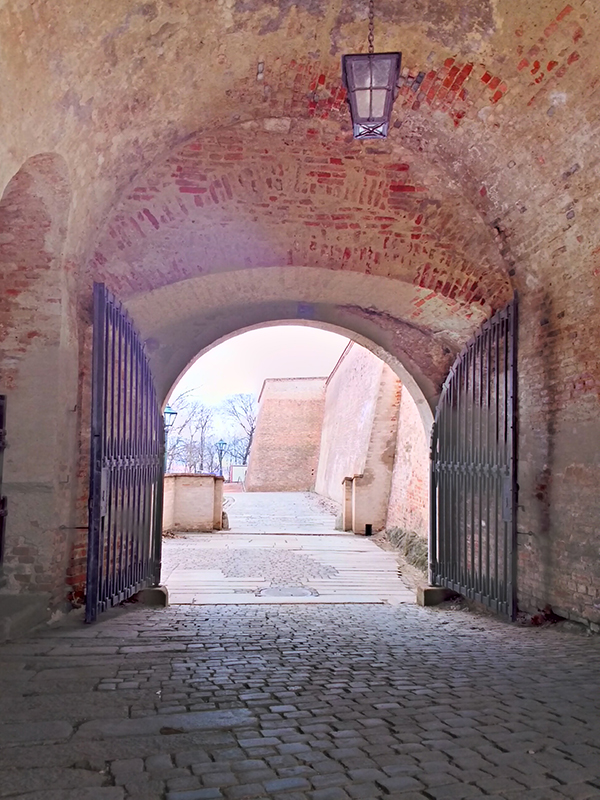
\includegraphics[width=\textwidth]{figures/tests/hdrApps/hdrCamera}
        \caption{HDR Camera}
        \label{fig:apps_1}
    \end{subfigure}
    ~
    \begin{subfigure}{0.3\textwidth}
        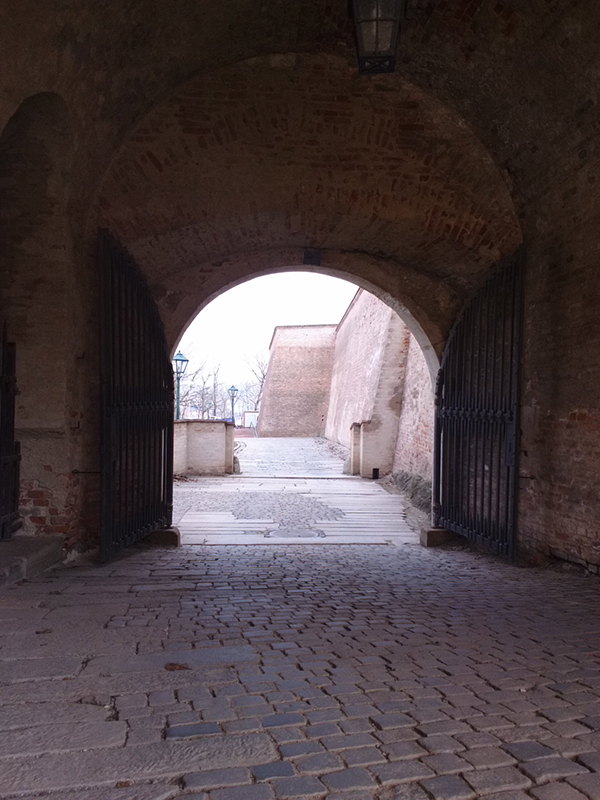
\includegraphics[width=\textwidth]{figures/tests/hdrApps/hdrHq}
        \caption{HDR HQ}
        \label{fig:apps_2}
    \end{subfigure}
    
    \begin{subfigure}{0.3\textwidth}
        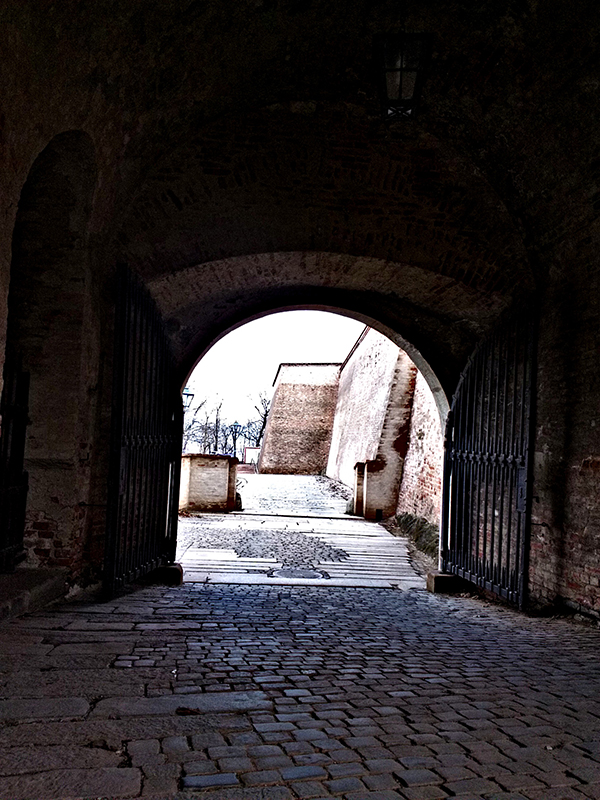
\includegraphics[width=\textwidth]{figures/tests/hdrApps/hdrMax}
        \caption{HDR Max}
        \label{fig:apps_3}
    \end{subfigure}
    ~
    \begin{subfigure}{0.3\textwidth}
        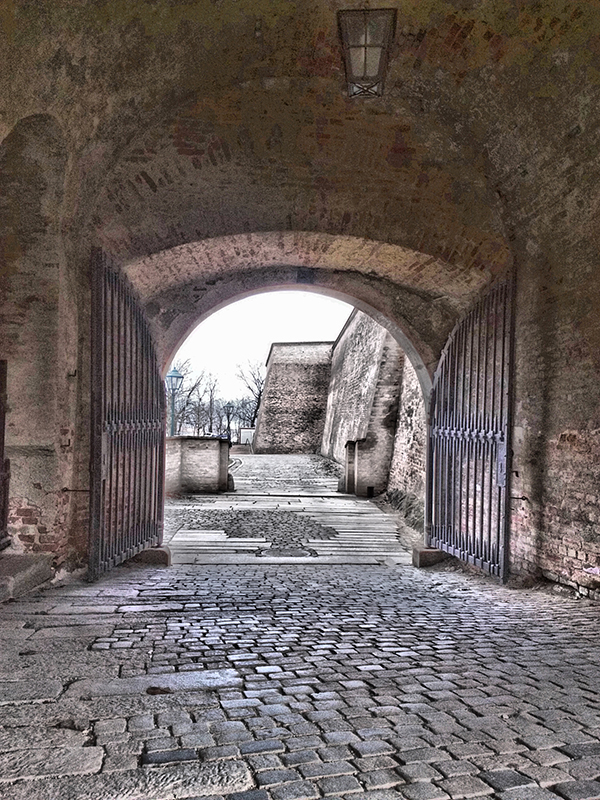
\includegraphics[width=\textwidth]{figures/tests/hdrApps/ultimateHdrCamera}
        \caption{Ultimate HDR Camera}
        \label{fig:apps_4}
    \end{subfigure}
    \caption{Scéna brány zachytená voľne dostupnými HDR aplikáciami}
    \label{fig:apps}
\end{figure}

Ako už bolo spomínané v prieskume existujúcich riešení, veľa aplikácií používa na vytvorenie HDR efektu
iba filter aplikovaný na jednu fotografiu, ktorý zvýši kontrast a detaily fotografie. Bez preskúmania
zdrojového kódu aplikácií je ťažké rozoznať či ide o 'pravé' HDR snímky alebo iba takúto napodobeninu.
Z prieskumu aplikácií boli vybrané najzaujímavejšie riešenia, ktorými bola zachytená scéna \textit{brana}.

Začneme najzaujímavejším výsledkom, ktorý vytvorila aplikácia Ultimate HDR Camera (obr. \ref{fig:apps_4}).
Na tomto obrázku môžeme vidieť jasného zástupcu fotografií, ktoré si užívateľ predstavuje pod pojmom
"HDR fotografia". Okrem umeleckého zážitku, ktorý výsledná fotografia ponúka zvýraznením detailov
a farieb, môžeme vidieť, že fotografia kvalitne zobrazuje svetlé aj tmavé oblasti scény. To znamená,
že vytvára viacero snímok s dostatočným rozsahom expozičného času. Z výsledku je rozpoznateľné, že sa jedná
o lokálny operátor, ktorý okrem mapovania tónov pracuje aj s farbami a kontrastom fotografie. Podobný
výsledok by sa nám pravdepodobne nepodarilo dosiahnúť v našej aplikácii, avšak treba poznamenať,
že ani jedna z fotografií (obr. \ref{fig:apps}) nemá dostatočný dynamický rozsah na to, aby nepreexponovala
oblohu v pozadí. Vo výsledkoch našej aplikácie sú vo všetkých operátoroch zachované farby oblohy.

Aplikácia HDR Camera (obr. \ref{fig:apps_1}) ponúka taktiež uspokojivý výsledok, z ktorého možno usúdiť,
že zahŕňa dostatočný dynamický rozsah scény a je použitý lokálny operátor. Pri bližšom pohľade však vidíme,
že na obrázku sa nachádzajú škvrny - miesta, na~ktorých sa stráca farebnosť. Príčina tohoto javu však nie je
objasnená. Podobný výsledok sme schopný v našej aplikácii dosiahnúť Durandovým operátorom.

Aplikácie HDR HQ (obr. \ref{fig:apps_2}) a HDR Max (obr. \ref{fig:apps_3}) sú príkladom riešení, ktoré nezachytávajú
väčší dynamický rozsah scény, ale snažia sa vytvoriť HDR efekt pomocou filtra.
